\section{Method}\label{sec:Method}


\subsection{Code Implementation}
Extending the previous \textsf{Scattering.jl} library to handle the potentials
spawned by effective field theory is a simple matter. Each potential corresponds
to a struct with the necessary coefficients, along with a callable method for
evaluating the potential. These are shown in~\cref{lst:eftpotential}.


\begin{listing}
\begin{minted}[linenos,mathescape=true,fontsize=\tiny,breaklines,escapeinside=||]{julia}
#= EFT Potentials =#
#= Lowest leading order pionless EFT potential =#
struct LO <: Potential
    C₀::Float64
end

function (V::LO)(k, k′)
    V.C₀
end

#= Next-to-leading order pionless EFT potential =#
struct NLO <: Potential
    C₀::Float64
    C₂::Float64
end

function (V::NLO)(k, k′)
    V.C₀ + V.C₂*(k^2 + k′^2)
end

#= Next-to-next-to-leading order pionless EFT potential =#
struct NNLO <: Potential
    C₀::Float64
    C₂::Float64
    C₄::Float64
    C₄′::Float64
end
NNLO(c0, c2, c4) = NNLO(c0, c2, c4, c4)

function (V::NNLO)(k, k′)
    V.C₀ + V.C₂*(k^2 + k′^2) + V.C₄*(k^4 + k′^4) + V.C₄′*k^2*k′^2
end
function (V::NNLO)(k, k′)
    V.C₀ + V.C₂*(k^2 + k′^2) + V.C₄*(k^4 + k′^4) + V.C₄*k^2*k′^2
end


#= Pion interaction =#
struct Pion <: Potential
    mπ::Float64
    Vπ::Float64
end
Pion(Vπ::Real) = Pion(0.7, Vπ)

function (V::Pion)(k, k′)
    mπ = V.mπ
    V.Vπ/(4mπ * k*k′) * log((mπ^2 + (k+k′)^2)/(mπ^2 + (k-k′)^2))
end

\end{minted}
\caption{Implementation of the EFT potentials.\label{lst:eftpotential}}
\end{listing}

Adding one-pion exchange term to the pionless potentials is done by a combining
a pionless potential with the one-pion exchange potential through a
\textsf{CompoundPotential}, its implementation shown in~\cref{lst:compoundpotential}.


\begin{listing}
\begin{minted}[linenos,mathescape=true,fontsize=\tiny,breaklines,escapeinside=||]{julia}
struct CompoundPotential <: Potential
    V1::Potential
    V2::Potential
end

function(V::CompoundPotential)(r)
    V.V1(r) + V.V2(r)
end

function(V::CompoundPotential)(k, k′)
    V.V1(k, k′) + V.V2(k, k′)
end

+(V1::Potential, V2::Potential)::Potential = CompoundPotential(V1, V2)

\end{minted}
\caption{Potentials can be combined, yielding a \textsf{CompoundPotential}. This
is used to easily add a one-pion exchange term to other potentials.
\label{lst:compoundpotential}}
\end{listing}

Finally, a potential can be regularized with the smooth UV regulator [ref] by
sandwiching a potential with the \(f_{\Lambda}\) factors, as implemented in~\cref{lst:uvregulator}.

\begin{listing}
\begin{minted}[linenos,mathescape=true,fontsize=\tiny,breaklines,escapeinside=||]{julia}
#= UV Regulatization =#
struct UVRegulator <: Potential
    V::Potential
    Λ::Float64  # Cutoff parameter [fm⁻¹]
end

function (V::UVRegulator)(k, k′)
    exp(-k^4/V.Λ^4) * V.V(k, k′) * exp(-k′^4/V.Λ^4)
end
\end{minted}
\caption{Regularization is too a \textsf{Potential} wrapped around another \textsf{Potential}.\label{lst:uvregulator}}
\end{listing}

\subsection{Minimization Procedure}

Earlier works on the same topic\cite{lepage1997renormalize,MACHLEIDT20111} often skimp on
detailing the methods used
to obtain the coefficients for the potentials. As a counterweight, the following is
a detailed explanation of the minimization employed here. Modern works are of
course much more detailed, but the methods they use are also too advanced to be
employed here.

\subsubsection{Region of Fit}
Potentials derived from effective field theory are most accurate at low
energies, i.e. the low infrared region. By construction, a fit here should give
the best overall fit for all energies. However, the phase
shift of the Reid potential is near linear for \(E<5\) MeV, before the peak. The
more degrees of freedom a parameterized potential has, the more trouble minimization
procedures will have in finding good coefficients that generalize without
being able to see more features. It is therefore to expect that potentials with
more degrees of freedom require data from higher and higher energies to perform
a good fit.

Fitting to higher energies is undesirable as the EFT potentials quickly break
down. In an effort to weight low energy points more, a bias is introduced using logarithmically spaced points
to put more weight on points with low energy. We will examine the effect of
fitting to different energy regions by changing the final energy
\(E_{\mathrm{end}}\) while holding \(\Lambda\) constant and examining the effect
on the quality of the fit.

\subsubsection{Fitting Error}
Any form of fitting procedure require a measure of the error. A common measure
is the square of the residuals, \(\left( y_{i} - \mathrm{fit}_{i} \right)^{2}\), used
in least squares and \(\chi^{2}\) minimization. This is not necessarily optimal
for our problem because the potentials derived from EFT are asymptotically good
as \(k\to 0\), and so one would expect the fit to get progressively worse as the
energy increases. If the square of the residuals is used, the error at high energies
will be weighted considerably more
than the error at low energies, biasing the fit for a better ``global'' fit. A
better choice might be to use the absolute error of the residuals
\(|y_{i}-\mathrm{fit}_{i}|\) as suggested by Lepage\cite{lepage1997renormalize}, or the relative error
\(\frac{|y_{i}-\mathrm{fit}_{i}|}{y_{i}}\). However, many standardized solvers
rely on the properties of the square of the residuals to perform their
minimization. We instead have to supply our own error function calculating the
relative error and select a
solver that tries to minimize this error.

This sends us to the problem of which minimization procedure to use. As we are
using the Reid potential as the \textit{Truth}, we need not care for empirical errors,
only about obtaining a good fit in a reasonable amount of time. This turns out
to be substantially more difficult than what it seems at face value. There are
two reasons for this. The first is that the dimension of the parameter space increases 
from \(1\) for LO to \(4\) with \(\mathrm{NNLO}\). Adding the pionic interaction
adds another parameter. Not only does this
make the solution space more shallow, it also introduces several
local minima. Having obtained one solution, one can not set aside the fear that
the solution is suboptimal, and many methods make it difficult to measure how
much of the parameter space one has explored. Trials showed that gradient-based
methods easily get stuck and several methods using exorbitant amount of time to
obtain convergence. Simulated annealing found very good fits, but only
after running for hours.

Another problem arises from the K-matrix method used to compute the phase shift.
There is an inherent limitation to the method as the computation of \(\delta\)
perform an \(\atan\), setting an upper bound of \(\pi/2\). Unfortunate values of
the parameters or their combination leads to discontinuous jumps in the phase
shift, which in turn causes the error to jump. The solvers I tried had
difficulties dealing with this. The situation was improved by modifying
the error function when noticing a jump in the phase shift to instead use
\begin{equation*}
  \Delta(\delta_{\text{reid}}, \delta) = \left| p\cdot\cot\left( \delta_{\text{reid}}(p) \right) - p\cdot\cot\left( \delta(p) \right)\right|
\end{equation*}
as suggested by\cite{steele1998regularization,taylor}. This lifts the degeneracy
in \(\delta\), but as it multiplied by the momentum \(p\), larger momenta will
weight considerably more. The intent is to steer the minimization procedure away
from parameters causing jumps in a smooth fashion to prevent it from getting stuck.

\subsubsection{Hyperparameters}

Among the choices when performing the fit is how many points to include.
 \cref{fig:fitpoints} shows the
relationship between the error in the fitting and number of points used for NLO,
as well as the time usage. As for all fitting methods, using more points will
reduce to error in the fit, but rather surprisingly the error increases rapidly
when the number of points goes below \(\approx 50\). The reason seems to be the
minimization struggling to achieve convergence. This is a bit worrying as
Lepage\cite[p.~35]{lepage1997renormalize} used only 2 points, but no change I
could come up with improved the situation.

The time usage is stochastic, tending to use more time when more points are used
and when the number of fit parameters increase.
The effect of number of points
on the coefficients are shown in \cref{fig:coefffitpoints} along with
bands showing the error relative to the coefficients from fitting with \(200\)
points. The first coefficient is within \(1\%\) after \(25\) points, while the
second requires \(50\) points to be within \(10\%\) of the best estimation. The
ideal number of points seem to be about \(50\), but this causes NLO and NNLO to
take an impractical amount of time to fit. As such, accuracy is sacrificed, and
\(10\) points are used hereon unless otherwise states. 

\begin{figure}[pt]
  \centering
  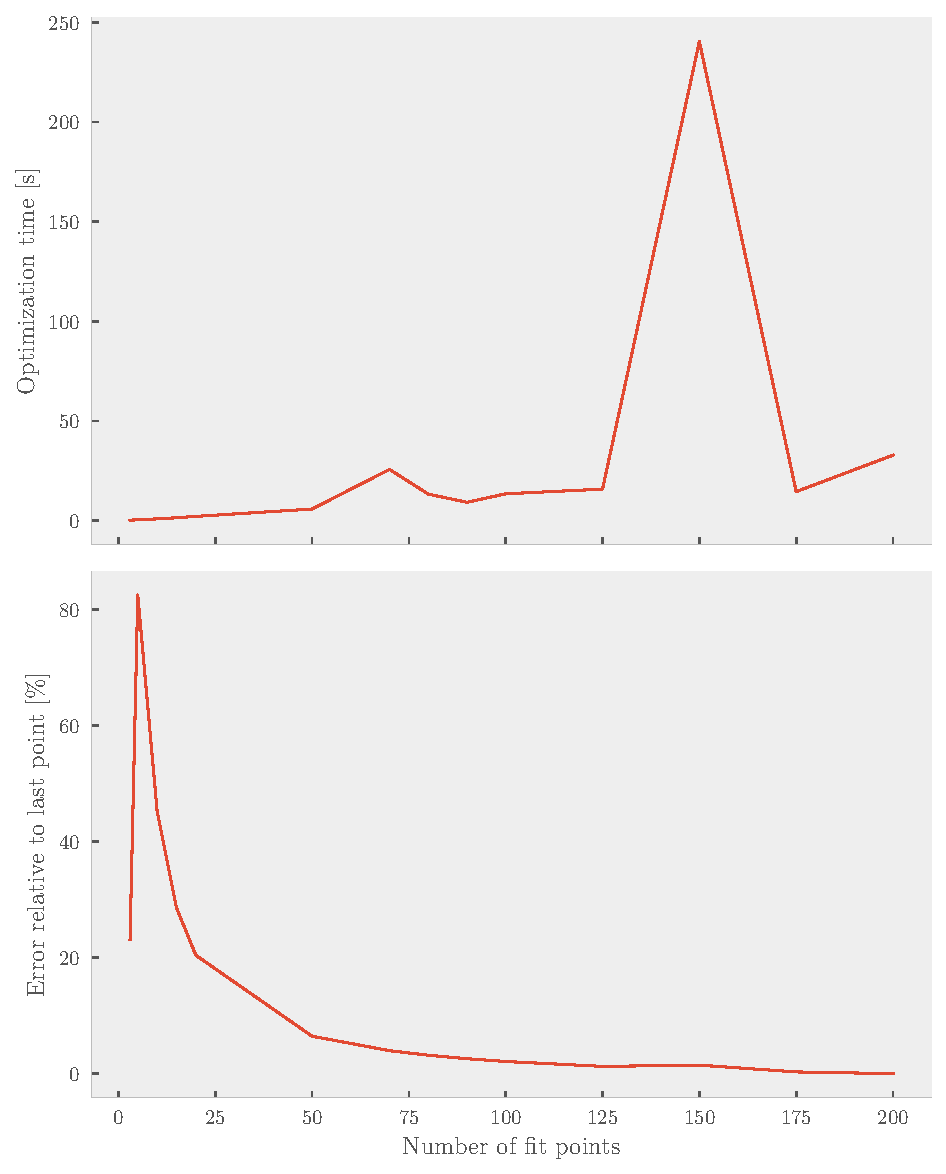
\includegraphics{Figures/NLO_dependence_time_error.pdf}
  \caption{\label{fig:fitpoints} The error (lower panel) in fitting NLO using a varying number
  of fitting points, as well as the time usage (top panel). The error is
  relative to the fitting from using 200 points. With \(\approx 50\)
  points the error is within \(10\%\), and increasing the number of points yield
only incremental improvement. The time usage is difficult to measure due to its
stochastic nature. The top panel only shows an example which is rather
unrepresentative. In general, the time increases significantly beyond \(\approx
20\) points, especially as the model complexity increases.}
\end{figure}

\begin{figure}[pt]
  \centering
  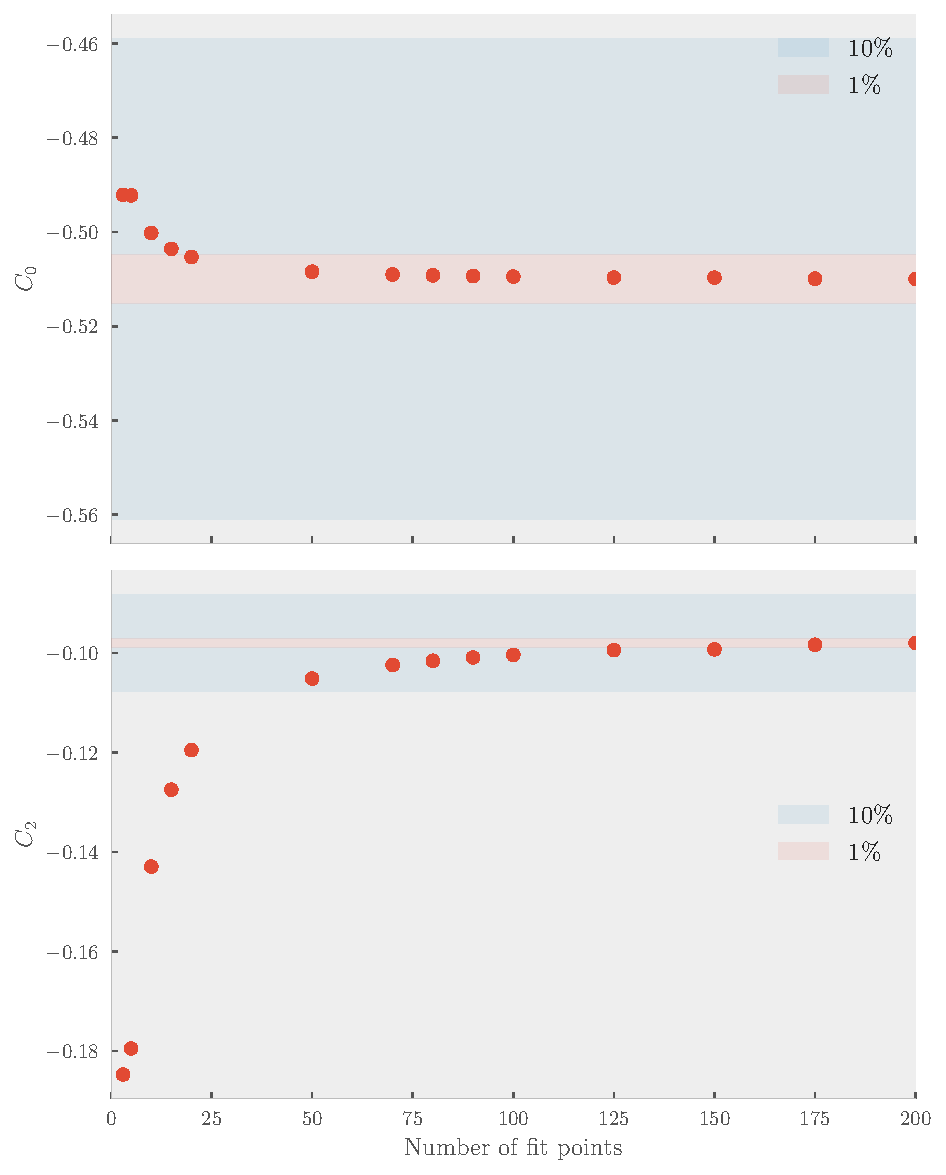
\includegraphics{Figures/NLO_coeff_dependence.pdf}
  \caption{\label{fig:coefffitpoints} The dependence of the coefficients on the
    number of points used in the fit. The bands show the error relative to the
    final result using \(200\) points. The points quickly converge as the
    number of points increase beyond \(\approx 50\).}
\end{figure}

\newpage

\subsection{Finding Optimal Cutoff}

The main goal is to find the optimal value of the cutoff parameter \(\Lambda\)
for the different models. From the theory we expect that the models without a
pion term will achieve their best result below \(\Lambda=m_{\pi}\). Including a
pion term will allow the models to account for simple pion exchange physics, and
 should be best at some value \(\Lambda > m_{\pi}\). To explore whether this is
 borne out by calculations, the potentials are fitted with different values of
 \(\Lambda\) in the range \(50\) to \(\approx 400\) MeV. 

When fitting the models, I had considerable difficulties with convergence. A
tell-tale sign of convergence is that the parameters vary smoothly with
\(\Lambda\). To help
the algorithm along, I extrapolated the model parameters from where it achieved
convergence into the region where it had problems, squeezing the bounds as
\(\Lambda\) increased. This worked well for LO and NLO, but only passably for
NNLO. 


\subsection{Problems}
The potentials are fitted to phase shifts generated by the Reid potential, but this introduces some
subtle systematic errors. The Reid potential is a phenomenological NN potential
composed of a sum of Yukawa interactions, not taking chiral or other symmetries into
account. No matter how good its coefficients are fit to data, the potential can
never achieve better accuracy than a sufficiently developed EFT potential. Reid (and later improvements) sought the best \textit{gloabl}
fit by minimizing \(\chi^{2}\) on the entire energy range, weighting by only the
errors in the data. This neglects the fact that effective field theories scale
with \((Q/\Lambda_{\chi})^{\nu+1}\). When we use Reid to fit our EFT potential,
it is therefore not to expect the errors we obtain to scale as nicely as it
would have, had direct experimental observables been used instead.

\FloatBarrier{}
%%% Local Variables:
%%% mode: latex
%%% TeX-master: "../main"
%%% TeX-engine: xetex
%%% End:
